%  Typ dokumentu - článek, prezentace aj.
\documentclass[english]{article}

%  Nastaví vstupní a výstupní kódování znaků (encoding) a lokalizace
\usepackage[T1]{fontenc}
\usepackage[utf8]{inputenc}
\usepackage[english,czech]{babel}
\usepackage{icomma}

%  Formát papíru a odsazení od jeho okrajů
\usepackage[letterpaper]{geometry}
\geometry{verbose,tmargin=1.5cm,bmargin=2cm,lmargin=2cm,rmargin=2cm}

%  Umožňuje pracovat s grafikou
\usepackage{graphicx}
\usepackage{bigstrut}
\usepackage{epstopdf}

%  Automaticky odsadí i první paragraf v každé sekci
\usepackage{indentfirst}

%  Umožňuje rozdělovat obsah na více sloupců
\usepackage{multicol}
\usepackage{booktabs}
\usepackage{pgffor}

%  Umožňuje používat hypertextové odkazy, nastavuje jejich barvu a vlastnosti
\usepackage[unicode]{hyperref}
\hypersetup{
	colorlinks=true, citecolor=blue, filecolor=blue, linkcolor=blue,
	urlcolor=blue
}

%  Umožnění odstranění italiky u jednotek
\newcommand{\unit}[1]{\mathrm{#1}}

%  Formátování stránek, empty = odstraní číslování
% \pagestyle{empty}

%  Řádkování
\linespread{1.2}

%  Lepší zobrazování matematiky (rozšíření sum o \limits atd.)
%  Umožní psát přes \mathbb{N/R/Q/..} množiny čísel
\everymath{\displaystyle}
\usepackage{amsmath, amsthm, amssymb, wasysym}

%  Velikost fontu matematických výrazů v dokumentu lze pro danou
% základního fontu dokumentu upravit pomocí:
% \DeclareMathSizes{X}{Y}{Z}{U} kde:
% X je velikost fontu v dokumentu, pro kterou se matematika upraví
% Y je standartní velikost fontu matematiky
% Z je velikost fontu zmenšených (vnořených výrazů)
% U je velikost fontu ještě více zmenšených (vnořených výrazů).
\DeclareMathSizes{10}{10.5}{9}{9}

%  Nastaví autora, název, datum, skupinu měření apod. 
%  (můj vlastní příkaz, umožní znovu-použití v dokumentu)
\newcommand{\Author}{David Roesel}
\newcommand{\Coauthor}{Schönfeldová, Vyšín}
\newcommand{\Institute}{FJFI ČVUT v Praze}
\newcommand{\Subject}{VAKUOVÁ FYZIKA A TECHNIKA}
\newcommand{\Group}{Pá 14:30}
\newcommand{\Kruh}{FE}
\newcommand{\Title}{Úloha \#1  \\Čerpání rotační olejovou vývěvou}
\newcommand{\Date}{7.11.2014}

% Custom comands
\newcommand{\dd}{\mathrm{d}}
\newcommand{\dln}{\mathrm{ln}}
\newcommand{\ee}{\mathrm{e}}
\newcommand{\jelina}{Oooo, Jelina!}

% Začátek dokumentu - Formátování na výstup
\begin{document}

% Interní proměnné, možno zobrazovat u prezentací, používají se při
% generování pomocí \titlepage apod.
\author{\Author}
\title{\Title}
\date{\Date}

%  Lokalizace některých názvů do češtiny
\renewcommand{\figurename}{Obr.}
\renewcommand{\tablename}{Tab.}
\renewcommand{\refname}{Reference}

% --- Hlavička dokumentu -----------------------------------------------

\setlength{\parindent}{0cm}
\begin{multicols}{2}
\textbf{\Subject \\
        \Institute \\[0.1cm]
%\large  \Title \\[0.5cm]
\Title \\[0.5cm]
}
\begin{tabular}{rlrl}
\large Datum měření: & \Date & \large Skupina: & \Group \\
\large Jméno: & \Author & \large Kroužek:  & \Kruh\\
\large Spolupracovali: & \Coauthor &\large Klasifikace:\\
\end{tabular}

\begin{flushright}

\includegraphics[scale=0.28]{../../_meta/fjfi_standart.pdf}
\hspace{0.2cm}
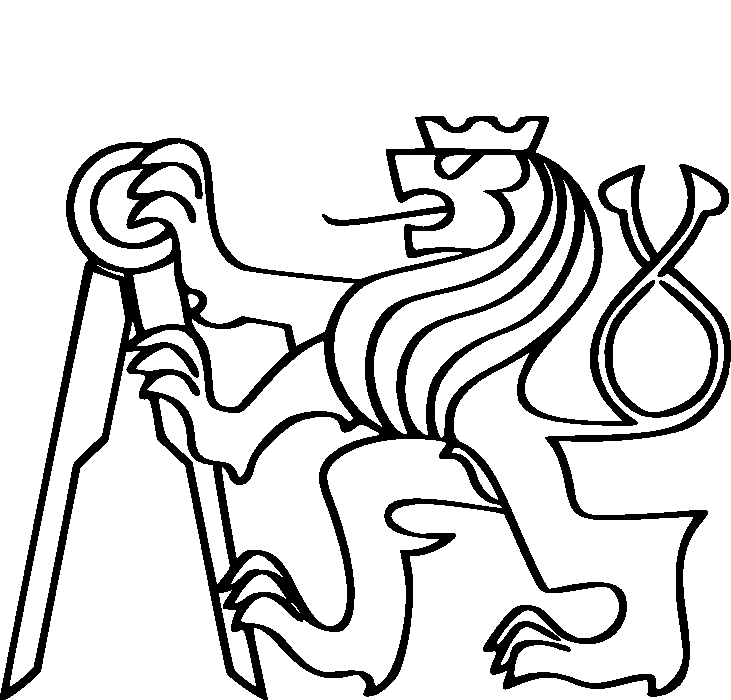
\includegraphics[scale=0.28]{../../_meta/cvut_standart.pdf}
\end{flushright}
\end{multicols}
\hrule
\vspace{0.5cm}

% ----------------------------------------------------------------------


% --- Tělo dokumentu ---------------------------------------------------
\setlength{\parindent}{0.5cm}

\section{Pracovní úkoly}
\begin{enumerate}
	\item Sledujte čerpání uzavřeného objemu rotační olejovou vývěvou (ROV)
	s uzavřeným a otevřeným proplachováním, a to od atmosferického tlaku
	až po přibližný mezní tlak. Ze závislosti $\unit{ln}p=\unit{f}(t)$ určete
	čerpací rychlost. 
	\item Určete čerpací rychlost z měření proudu plynu (mikrobyretou) při konstantním
	tlaku. Proveďte pro tři hodnoty tlaku od 5 do 20 Pa. 
	\item Určete, jak ovlivňuje efektivní čerpací rychlost hadice mezi ROV a
	recipientem. 
	\item Ocejchujte termočlánkový vakuometr v rozsahu 6 až 30 dílků sklápěcím
	kompresním vakuometrem McLeod (cca 10 bodů). 
	\item Měřením tlakového spádu (termočlánkovým vakuometrem a McLeodem) a
	proudu vzduchu (mikrobyretou) určete vodivost kovové trubice ($\diameter=8,5~\unit{mm},\ l=100~\unit{cm}$)
	pro vstupní tlaky od 5 do 50 Pa. Určete vodivost trubice výpočtem
	a výsledky srovnejte. 
\end{enumerate}

\section{Úvod}

Rotační olejová vývěva (ROV) je mechanická transportní vývěva. Rotační olejové vývěvy typicky dosahují
tlaků v řádu jednotek Pascalů bez proplachování, s proplachováním
potom tlaků o dva řády vyšších. 

V rotačních olejových vývěvách se dosahuje poměrně vysokého kompresního
poměru, což může pro plyny s vysokou kritickou teplotou vést k jejich
zamíchání do oleje, který se tím znehodnotí, jelikož se pak z oleje
v nežádaných místech aparatury plyn může opět uvolňovat. Zabraňuje
se tomu používáním tzv. proplachování, které vede k tomu, že se výstupní
ventil otevírá dříve, než by stihlo vlivem tlaku dojít ke kondenzaci
par. V experimentu se budeme snažit ověřovat, že proplachování opravdu
zvyšuje mezní tlak vývěvy o jeden až dva řády. 

\section{Vypracování}
  \subsection{Teoretický úvod}				
	\subsubsection{Čerpací proces ROV}
	
	Čerpáme-li pomocí rotační olejové vývěvy recipient a sledujeme-li
	tlak, využijeme následující vztahy:
	\begin{equation}
	q = pS = p\frac{\dd V}{\dd t} = -V\frac{\dd p}{\dd t},
	\label{cerpane_mnozstvi}
	\end{equation} 
	
	
	kde $q$ je zdroj plynu (netěsnost), $V$ čerpaný objem, $p$ tlak
	a $t$ čas. Snadnou úpravou se pak dostaneme k finální podobě vzorce
	\begin{equation}
	S=-V\frac{1}{p}\frac{\dd p}{\dd t}=-V\frac{\dd\ln p}{\dd t}.\label{eq:lnp}
	\end{equation}
	
	Z teorie pro nás bylo také důležité vědět, že dotyky po sobě klouzajících
	částí a výstupní ventil nejsou dokonale těsné a olej jimi prolíná,
	což nevadí za provozu, kdy je neustále hnán ven z výstupu. Pokud by
	ale rotační olejová vývěva neběžela a ve vstupním hrdle by zůstal
	snížený tlak, byl by olej nasáván rozdílem tlaků a mohl by se dostat
	až do čerpaného objemu, což by vedlo ke znečištění aparatury. Po jejím
	vypnutí bylo tedy třeba rotační vývěvu zavzdušnit vhodným přepnutím
	jejího ventilu.
		
	\subsubsection{Měření čerpací rychlosti při konstantním tlaku}
	
	Dále budeme potřebovat měřit efektivní čerpací rychlost při konstantním
	tlaku. Vycházíme přitom z kontinuity proudění, tedy z rovnosti mezi
	proudem plynu čerpaného rotační vývěvou a proudem plynu napouštěného
	do aparatury. Zapíšeme-li tuto rovnost matematicky, dostáváme
	\begin{equation}
	S_{EF}(p)\cdot p=q=p_{A}\frac{\delta V}{\delta t},\label{eq:Sef}
	\end{equation}
	
	
	kde $\delta V$ je objem vzduchu odsátý z mikrobyrety za čas $\delta t$,
	$p$ tlak v místě určování efektivní čerpací rychlosti $S_{EF}$,
	$q$ proud vzduchu a $p_{A}$ atmosferický tlak. Hodnoty poměru $\frac{\delta V}{\delta t}$
	budeme určovat vzorcem 
	\begin{equation}
	\frac{\delta V}{\delta t}=\frac{l}{\tau}\cdot4,75\cdot10^{-2}\qquad\unit{[cm;s;\frac{{cm^{3}}}{s}]},\label{eq:dV/dt_empiric}
	\end{equation}
	
	
	uvedeným na mikrobyretě. Veličina $l$ je délka, o kterou vystoupala
	kapalina v mikrobyretě za čas $\tau$.
	
	
	\subsubsection{Vliv hadice na čerpací rychlost}
	
	Střední volnou dráhu molekuly ve vzduchu za normálních podmínek můžeme
	určit ze vztahu
	\begin{equation}
	l_{s}=6,6\cdot10^{-3}\cdot\frac{1}{p}\qquad\unit{[m;Pa]},
	\label{eq:ls}
	\end{equation}
	
	
	kde $p$ je tlak. Pravděpodobná rychlost pohybujících se částic $v_{p}$ je definována
	jako
	\begin{equation}
	v_{p}=\sqrt{\frac{2kT}{m}},\label{eq:v_p}
	\end{equation}
	
	
	kde $T$ je teplota, $m$ je hmotnost částice. Vztah pravděpodobné
	rychlosti $v_{p}$ a střední rychlosti $v_{s}$ je 
	
	\begin{equation}
	v_{s}=1,128\cdot v_{p}.\label{eq:vs_vp}
	\end{equation}
	
	
	Hmotnost částice vzduchu můžeme získat za znalosti molární hmotnosti
	molekul vzduchu $M_{m}$ a Avogadrovy konstanty $N_{A}$ pomocí vzorce
	\[
	m=\frac{M_{m}}{N_{A}}.
	\]
	
	
	Hodnotu molární hmotnosti molekul vzduchu uvažujeme $M_{m}=28,96~\unit{g\cdot mol\cdot10^{-1}}$.
	Dosadíme-li tento vzorec do vztahu (\ref{eq:vs_vp}) a ten následně
	do (\ref{eq:v_p}), získáme pro střední rychlost částice vztah
	\begin{equation}
	v_{s}=1,128\cdot\sqrt{\frac{2RT}{M_{m}}},\label{eq:vs}
	\end{equation}
	
	
	kde $R$ je plynová konstanta. Vodivost trubice, která je dlouhá $l$
	a má průměr $\diameter$, můžeme za podmínek viskózně molekulárního
	proudění vypočítat podle empirického vzorce \cite{bib:praskripta}
	\begin{equation}
	C=\frac{\pi\diameter^{2}}{4}\frac{\diameter}{l}\left[\frac{\pi}{128}\frac{\diameter}{l_{s}}+\frac{{1}}{3}\frac{{2+2,057\frac{{\diameter}}{l_{s}}}}{2+3,095\frac{{\diameter}}{l_{s}}}\right]\cdot v_{s}.
	\label{eq:Cvm}
	\end{equation}
		
	\subsubsection{Měření pomocí McLeodova manometru}
	
	Měření tlaku McLeodovým manometrem je přímé a platí vzorec uvedený
	v dokumentaci přístroje u experimentu
	\begin{equation}
	p=\frac{133,3\cdot lh}{1100-l}\qquad\unit{[Pa;mm;mm]},\label{tlak}
	\end{equation}
	
	kde $l$ je vzdálenost mezi vrchem uzavřené trubice a hladinou v ní
	a $h$ je rozdíl hladin. 
	
	\subsubsection{Měření vodivosti trubice}
	Pro vodivost trubice $ C $ s tlaky na koncích $ p_1 $ a $ p_2 $ platí
	\begin{equation}
	C = \frac{q}{p_1 - p_2},
	\label{vodivost_trubice}
	\end{equation}
	kde $ q $ je proud plynu, který je dán vztahem 
	\begin{equation}
	q = p_A\cdot \frac{\delta V}{\delta t},
	\label{proud}
	\end{equation}
	kde veličina $ \mathrm{\frac{\delta V}{\delta t}} $ je dána vztahem (\ref{eq:dV/dt_empiric}).\\
	
	Průměrný tlak $ p_s $ v trubici lze určit ze vztahu
	\begin{equation}
	p_s = \frac{p_1 + p_2}{2},
	\label{pruměr_tlak}
	\end{equation}
	kde $ p_1 $ je tlak na vstupu a $ p_2 $ tlak na výstupu trubice.
			
\subsection{Postup měření}

	\subsubsection{Čerpací proces ROV}
	
	Zkontrolovali jsme, že aparatura je sestavena dle schématu na Obr. \ref{schema1}. Aparaturu jsme odšroubováním rychlospoje, který spojoval recipient s Piraniho manometrem, napustili vzduchem na atmosferický tlak. Poté jsme ji uzavřeli, spustili Piraniho manometr a zapnuli ROV. V okamžiku otevření ventilu, který vedl z ROV do recipientu, jsme začali měřit čas. Sledovali jsme, jak se s časem mění tlak v recipientu a zaznamenávali jej. Totéž měření jsme provedli pro ROV s proplachováním.
	
	\subsubsection{Měření čerpací rychlosti při konstantním tlaku}
	Čerpací aparaturu jsme nechali zapojenou dle schématu na Obr.~\ref{schema1}. Aparaturu jsme vyčerpali pomocí ROV bez proplachování a snažili se za pomoci jehlového ventilu docílit konstantního tlaku $ 5 $ Pa. Po ustálení tlaku jsme odaretovali mikrobyretu a měřili čas, za který vystoupil olej v mikrobyretě na hodnotu $ 10 $ cm. Celé měření jsme zopakovali ještě pro konstantní tlak $ 10 $ a $ 20 $ Pa.
	
	\subsubsection{Měření pomocí McLeodova manometru}
	Pro cejchování termočlánkového vakuometru jsme přestavili aparaturu dle schématu na Obr.~\ref{schema1}. Místo Piraniho manometru jsme umístili termočlánkovou měrku a místo, kde byla původně termočlánková měrka, jsme uzavřeli kovovou záslepkou. Vyčerpali jsme aparaturu a jehlovým ventilem jsme opět nastavili konstantní tlak na $ 9 $ dílků termočlánkového vakuometru. Otočili jsme McLeodův vakuometr a odečetli hodnoty hladin. Celé měření jsme provedli ještě desetkrát v rozmezí od 9 do 22 dílků.
	
				\begin{figure}[h!]
				\centering
				\begin{minipage}[t]{.40\textwidth}
				  \centering
								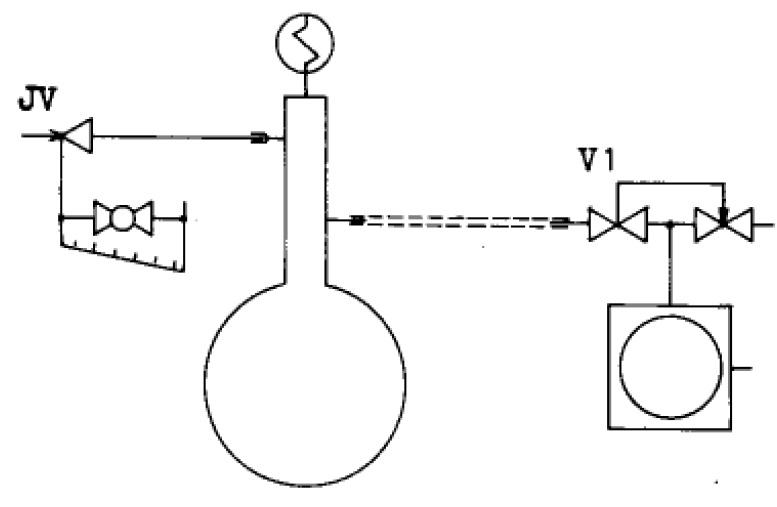
\includegraphics[scale=0.27]{../att/sch_cerpaci_rychlost}
								\caption{Schéma čerpací aparatury pro měření čerpacího procesu ROV a a její čerpací rychlosti - převzato z \cite{bib:praskripta}.}
								\label{schema1}
				\end{minipage}%
				\hfill
				\begin{minipage}[t]{.50\textwidth}
				  \centering
								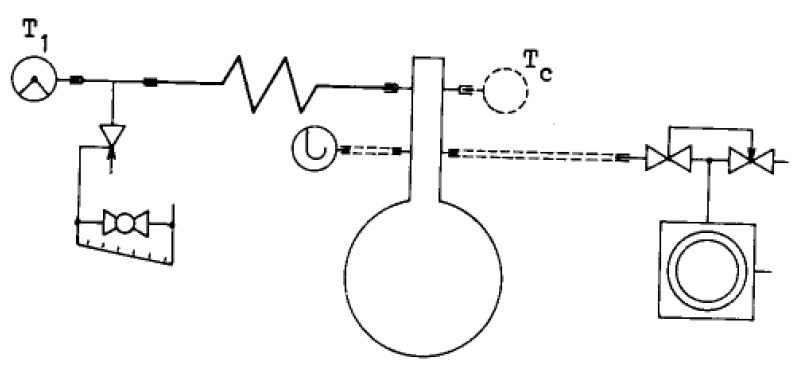
\includegraphics[scale=0.33]{../att/sch_vodivost_trubice}
								\caption{Schéma aparatury pro měření vodivosti trubice při viskózně molekulárním proudění - převzato z \cite{bib:praskripta}.}
								\label{schema2}
				\end{minipage}
				\end{figure}
	
	\subsubsection{Měření vodivosti trubice}
	Aparaturu jsme sestavili podle schématu na Obr.~\ref{schema2}. Jehlovým ventilem jsme nastavili konstantní tlak na termočlánkové měrce, poté jsme otočili McLeodovým vakuometrem a odečetli hodnoty. Dále jsme odaretovali mikrobyretu a měřili čas, za který olej vystoupil na hodnotu 10. Měření jsme provedli ještě pro 5 dalších hodnot tlaků.

\subsection{Naměřené hodnoty}
	
	\subsubsection{Čerpací proces ROV}
	
	Naměřené hodnoty jsou uvedeny v Tab. \ref{tlak1} a zobrazeny v grafech na Obr. \ref{lnp} a \ref{lnp_proplach}.
	Objem aparatury byl $ \mathrm{V} = 11,35~l$. 
	
	Pomocí fitování hodnot získaných při čerpání ROV bez proplachování v časovém rozmezí $ t = 0-250 $ s jsme získali směrnici
	\begin{equation}
	\frac{\dd(\dln \,p)}{\dd t} = (-0,038\pm0,001).
	\end{equation} 
	Čerpací rychlost jsme poté určili pomocí rovnice (\ref{eq:lnp}) jako
	\begin{equation}
	S_{uz} = (0,43\pm0,02) \, \mathrm{l\cdot s^{-1}}
	\end{equation} 
	s chybou dle (\ref{eq:chyba_neprime_mereni}).
	
	
	Pro čerpací rychlost s proplachováním pak v časovém rozmezí $ t = 0-350 $ s vyšla směrnice fitu 
	\begin{equation}
	\frac{\dd(\dln \,p)}{\dd t} = (-0,033\pm0,001) 
	\end{equation} 
	a čerpací rychlost tedy podle vztahu (\ref{eq:lnp}) jako
	\begin{equation}
	S_{ot} = (0,37\pm0,02)~\mathrm{l\cdot s^{-1}}
	\end{equation} 
	s chybou dle (\ref{eq:chyba_neprime_mereni}).
	
	\subsubsection{Měření čerpací rychlosti při konstantním tlaku}
	
	Naměřená data jsou uvedena v Tab. \ref{efektivni_cerpani}. Hodnotu atmosferického tlaku jsme brali z \cite{bib:tlak} jako $p_A = 101670~\unit{Pa}$. Hodnoty $ \frac{\delta V}{\delta t} $ jsme určili dle vztahu (\ref{eq:dV/dt_empiric}). Efektivní čerpací rychlost jsme poté spočetli za pomoci vztahu (\ref{eq:Sef}).
	
	\subsubsection{Vliv hadice na čerpací rychlost}
	Délku a průměr trubice spojující ROV s recipientem jsme brali jako $ l = (70\pm 1)~\unit{cm}$ a $ \diameter = (1,9 \pm 0,1)~\unit{cm}$ (chybu odhadujeme). Pro pět hodnot tlaků v rozmezí $ p = 5 - 25~\unit{Pa}$ jsme vypočítali střední volnou dráhu $l_s$ ze vztahu (\ref{eq:ls}). Z vypočtené hodnoty jsme zjistili, že se nejspíše jedná o viskózně molekulární proudění. Ze vztahu (\ref{eq:vs}) jsme stanovili střední rychlost molekul vzduchu pro teplotu $ T = 293 $ K, která činila $ v_s = 463~\unit{m/s}$. Pro dané tlaky jsme určili vodivost $C_{vm}$ této trubice pomocí vztahu (\ref{eq:Cvm}). Vypočítané hodnoty jsou uvedeny v Tab. \ref{tab:vodivost}. Závislost vodivosti trubice na tlaku v recipientu je vynesena v grafu na Obr. \ref{graf_vodivost} a proložena lineárním fitem. 
	
	\subsubsection{Měření pomocí McLeodova manometru}
	Naměřená data jsou uvedena v Tab. \ref{tab:cejchovani} a vynesena do grafu Obr. \ref{graf_cejchovani}. Tlak $ p $ jsme spočítali pomocí vzorce (\ref{tlak}).
	
	\subsubsection{Měření vodivosti trubice}
	Naměřená data se nachází v Tab. \ref{tab:vodivost2}. Na Obr. \ref{graf_vodivost2} je vynesena závislost naměřené a vypočítané vodivosti kovové trubice na středním tlaku. Hodnotu tlaku $p_1$ na vstupu trubice jsme spočítali ze vzorce (\ref{tlak}), hodnotu tlaku $p_2$ na výstupu jsme pak brali z hodnot získaných cejchováním termočlánkového vakuometru. Střední hodnotu tlaku jsme získali pomocí vzorce (\ref{pruměr_tlak}). Hodnoty naměřené vodivosti $C_{nam}$ jsme získali ze vztahu (\ref{vodivost_trubice}). Vodivost $C_{vm}$ jsme vypočítali vztahem (\ref{eq:Cvm}).

			
\subsection{Diskuse}
	\subsubsection{Čerpací proces ROV}
		Při sledování čerpání uzavřeného objemu jsme zjistili, že rotační olejová vývěva dosahuje s proplachováním horších tlaků než bez něj a to zhruba o jeden a půl řádu. To přesně odpovídá našemu předpokladu, který říká, že horší tlak vlivem proplachování je cenou za neznečištění oleje látkami, které by se do něj při vyšších tlacích zamíchaly. 
		
		I přes odpovídající rozdíl řádů tlaku při zapnutém a vypnutém proplachování musíme konstatovat, že jsme nedosáhli předpokládaných tlaků. U rotační olejové vývěvy by bylo rozumné očekávat tlak kolem 1 Pa, avšak naše zaznamenané minimum bylo těsně pod hodnotou 5 Pa. Jedním z důvodů mohly být netěsnosti v aparatuře, které mohly být přítomny již před naším příchodem k experimentu. Dvakrát za experiment nám vypadlo z některých spojů těsnění a je možné, že jsme způsobili menší netěsnost jeho nedostatečným očištěním. Další nezanedbatelný důvod bylo mírné přetočení (přenastavení) Piraniho měrky, která na začátku experimentu při atmosferickém tlaku ukazovala nesmyslně nízký tlak, takže ji bylo nutno vedoucím praktika jemně přenastavit. Tlak, kterého jsme dosáhli, tedy nemůžeme nazývat tlakem mezním.
		
		Lineární proložení naměřených dat jsme dělali na úseku $0-250$ sekund od zapnutí vývěvy, jelikož po tuto dobu působil průběh závislosti $\ln p = \unit{f}(t)$ lineárně. Námi určená čerpací rychlost by se rozhodně drobně změnila v případě, že bychom změnili interval, na kterém jsme hodnoty fitovali. Celou první část jsme navíc měřili na poměrně nepřesném Piraniho vakuometru, který nám dovoloval odečítat s rozumnou spolehlivostí pouze některé hodnoty a při automatickém přepínání rozsahů se někdy zasekával. Chyby naměřených hodnot tedy můžou být větší, než ty námi určené.
		
	\subsubsection{Měření čerpací rychlosti při konstantním tlaku}
		Při měření čerpací rychlosti při konstantním tlaku jsme zjistili, že efektivní čerpací rychlost $S_{EF}$ roste se stoupajícím tlakem, nikoliv však lineárně. Naměřené hodnoty by šly proložit parabolickou křivkou, ale vzhledem k malému množství určených hodnot by to nemělo valný smysl. Podařilo se nám ověřit, že efektivní čerpací rychlost byla pro každý tlak nižší než ta, kterou jsme určili v první úloze. 
		
		V jednom ze tří případů se některým z nás zdálo, že pohyb oleje v mikrobyretě nebyl konstantní, ale nepodařilo se nám tento jev znovu reprodukovat. Nejsme si také jisti, na kolik při větších čerpacích rychlostech ovlivnil rychlost stoupání oleje jeho zbytek z předešlého měření na spodku trubičky.
		
	\subsubsection{Vliv hadice na čerpací rychlost}
		Z grafu na Obr.~\ref{graf_vodivost} je zcela patrné, že v případě viskózně-molekulárního proudění roste vodivost trubice s tlakem lineárně. Dle našich výpočtů se zdá, že by vodivost hadice mezi recipientem a rotační olejovou vývěvou měla být dost vysoká na to, aby příliš neovlivňovala čerpací rychlost. Pokud bychom za ROV umístili vývěvu, která by byla schopna dosáhnout řádově lepších tlaků, bylo by možné, že by vodivost hadice snižovala $S_{EF}$ v limitě až k hodnotě $S_{EF}\approx C$. 
	
	\subsubsection{Měření pomocí McLeodova manometru}
		Vzhledem k tomu, že otočení jehlového ventilu mělo jistou latenci, nepodařilo se nám při měření pomocí McLeodova manometru ustálit tlak na žádné z hodnot. Ve výsledku jsme měření prováděli tak, že jsme otevřeli ventil natolik, aby se tlak měnil co nejpomaleji a čekali jsme, než ručička dojede na polohu, ve které jsme chtěli tlak ustálit. V ten moment jsme rychle provedli odečtení hodnot a postup s mírnou změnou natočení jehlového ventilu opakovali. Přesnost měření by šla zvýšit v případě, že bychom věnovali ustálení tlaku větší množství času.
		
		V jednom momentu jsme zapomněli otočit McLeodův manometr do původní polohy a nechali jsme klesnout tlak v aparatuře, což mělo za následek nahromadění rtuti v levé trubičce manometru. Opravování tohoto problému nás nějakou dobu zdrželo, ale předpokládáme, že jsme nijak neovlivnili žádná z následujících měření. K nepřesnostem však mohlo docházet při odečítání ze stupnic, konkrétně při přesném stanovování polohy hladiny v kapiláře. 
		
	\subsubsection{Měření vodivosti trubice}
		Vodivost trubice jsme určili výpočtem a měřením a můžeme říct jen to, že se hodnoty shodují řádově (jak je patrné z grafu na Obr.~\ref{graf_vodivost2}). Vzhledem k nedostatkům popsaným v předchozích bodech však řádovou shodu považujeme za dobrou. Pro přesnější porovnání by stálo za to provést cejchování termočlánkového vakuometru několikrát, jelikož jsme při něm brali hodnoty za absolutně přesné a adekvátně tomu jsme je místo fitu v grafu na Obr.~\ref{graf_cejchovani} propojovali. Při tomto měření navíc dělalo několik lidí na experimentu nezávisle na sobě a je možné, že každý měřil svoji část v jiném momentu. 
			
						
\section{Závěr}
	Sledovali jsme čerpání uzavřeného objemu rotační vývěvou (ROV) s uzavřeným a otevřeným proplachováním, a to od atmosferického tlaku až po tlak, který se ustálil na dostatečně dlouhou dobu (nemůžeme ho nazvat mezním). Ze závislosti $\ln p = \unit{f}(t)$ jsme určili čerpací rychlost jak pro uzavřené $S_{uz} = (0,43\pm0,02) \, \mathrm{l\cdot s^{-1}}$, tak pro otevřené $S_{ot} = (0,37\pm0,02)~\mathrm{l\cdot s^{-1}}$ proplachování. 
	
	Určili jsme čerpací rychlost z měření proudu plynu (mikrobyretou) při třech různých hodnotách konstantního tlaku.
	
	Určili a diskutovali jsme, jak hadice mezi ROV a recipientem ovlivňuje efektivní čerpací rychlost.
	
	Ocejchovali jsme termočlánkový vakuometr v rozsahu 6 až 30 dílků sklápěcím vakuometrem McLeod (cca 10 bodů).
	
	Měřením tlakového spádu (termočlánkovým vakuometrem a McLeodem) a proudu vzduchu (mikrobyretou) jsme určili vodivost kovové trubice pro několik vstupních tlaků. Vodivost trubice jsme určili výpočtem a výsledky jsme tabulkově i graficky srovnali.
	
	
\section {Použitá literatura}
% --- Literatura a reference -------------------------------------------
\begingroup
\renewcommand{\section}[2]{}

\begin{thebibliography}{9}

\bibitem{bib:chyby} Kolektiv KF, \emph{Chyby měření} [Online], [cit. \today] \newline http://praktikum.fjfi.cvut.cz/documents/chybynav/chyby-o.pdf

\bibitem{bib:praskripta}Král, J.: \emph{Cvičení z vakuové techniky},
Vydavatelství ČVUT, Praha, 1996

\bibitem{bib:tlak}ČHMÚ: \emph{Aktuální informace o počasí na území
České republiky}, {[}online{]}, {[}cit. \today{]},\\
 http://pr-asv.chmi.cz/synopy-map/pocasisp.php?ukazatel=stanice\&pozadi=\&pozadi=mapareg\&graf=ano
 

\end{thebibliography}
\endgroup
% ----------------------------------------------------------------------
\setcounter{equation}{0}
\numberwithin{equation}{section}

\clearpage
\part*{Přílohy}

%\section{Domácí příprava}
%	Domácí příprava je přiložena k protokolu.
%\clearpage
\section{Statistické zpracování dat}
	Pro statistické zpracování využíváme aritmetického průměru:
	\begin{equation} \label{eq:aritmeticky_prumer}
	\overline{x} = \frac{1}{n}\sum\limits_{i=1}^{n}x_i,
	\end{equation}

%	jehož směrodatnou odchylku spočítáme jako 
%	\begin{equation} \label{eq:smodch_aritmetickeho_prumeru}
%	\sigma_0 = \sqrt{\frac{1}{n} \sum\limits_{i=1}^{n}\left( x_i - \overline{x} \right)^2 },
%	\end{equation}
%	
%	kde $ x_i $ jsou jednotlivé naměřené hodnoty, $ n $ je počet měření, $ \overline{x} $ aritmetický průměr a $ \sigma_0 $ jeho chyba \cite{bib:chyby}.
	
	
	jehož chybu spočítáme jako 
	\begin{equation} \label{eq:chyba_aritmetickeho_prumeru}
	\sigma_0 = \sqrt{\frac{1}{n(n-1)} \sum\limits_{i=1}^{n}\left( x_i - \overline{x} \right)^2 },
	\end{equation}
	
	kde $ x_i $ jsou jednotlivé naměřené hodnoty, $ n $ je počet měření, $ \overline{x} $ aritmetický průměr a $ \sigma_0 $ jeho chyba \cite{bib:chyby}.
%	
Při nepřímém měření počítáme hodnotu s chybou dle následujících vztahů:
	\begin{equation}
	u = f(x, y, z, \ldots),
	\end{equation}
	\begin{displaymath}
	x = (\overline{x} \pm \sigma_x), \qquad
	y = (\overline{y} \pm \sigma_y), \qquad
	z = (\overline{z} \pm \sigma_z), \qquad
	\ldots,
	\end{displaymath}
	
	kde $ u $ je veličina, kterou určujeme nepřímo z měřených veličin $ x, y, z, \ldots $ 
	
	Pak
	\begin{displaymath}
	\overline{u} = f(\overline{x}, \overline{y}, \overline{z}, \ldots),
	\end{displaymath}
	\begin{equation}\label{eq:chyba_neprime_mereni}
	\sigma_u = \sqrt{\left( \frac{\partial f}{\partial x} \right)^2 \sigma^2_x + \left( \frac{\partial f}{\partial y} \right)^2 \sigma^2_y + \left( \frac{\partial f}{\partial z} \right)^2 \sigma^2_z + \ldots},
	\end{equation}
	\begin{displaymath}
	u = (\overline{u} \pm \sigma_ u).
	\end{displaymath}
%%	
%V případě, že máme několik různě přesných měření stejné veličiny, používáme vztah pro vážený průměr:
%	\begin{equation} 
%	\overline{x}=\frac{\sum\limits_{i=1}^{n}p_{i}x_{i}}{\sum\limits_{i=1}^{n}p_{i}},
%	\end{equation}
%	
%	kde $\overline{x}$ je vážený průměr, $x_{i}$ jsou jednotlivá měření a pro $p_{i}$ platí
%	 
%	\begin{equation}
%	p_{i}=\frac{1}{\sigma_{i}^{2}},
%	\end{equation}
%	
%	kde $\sigma_{i}$ jsou jednotlivé chyby daných měření.
%	 
%	Celkovou chybu tedy vypočítáme ze vztahu
%	\begin{equation} \label{eq:vazeny_prumer}
%	\sigma_{0}=\sqrt{\frac{1}{\sum\limits_{i=1}^{n}p_{i}}}.
%	\end{equation}
%
%\subsubsection{Metoda nejmenších čtverců}
%Snažíme-li se metodou nejmenších čtverců proložit data lineární závislostí $Y_i = ax_i+b$, dosazujeme hodnoty $x_i, y_i$ a snažíme se najít parametry $a$ a $b$ tak, aby byl součet všech kvadratických odchylek $\Delta Y_i^2$ minimální. Toho dosáhneme pomocí následujících vzorců \cite{bib:ctverce} :
%\begin{equation}\label{eq:ctverce_a}
%		a = \frac{n\sum\limits_{i=1}^{n}{x_i y_i}  - \sum\limits_{i=1}^{n}{x_i}\sum\limits_{i=1}^{n}{y_i}}{n\sum\limits_{i=1}^{n}{x_i^2}  - \left(\sum\limits_{i=1}^{n}{x_i}\right)^2}, \qquad \qquad
%		\sigma_a = \sqrt{\frac{n\sum\limits_{i=1}^{n}{(y_i - Y_i)^2} }{(n-2)\left(\sum\limits_{i=1}^{n}{x_i^2}  - \left(\sum\limits_{i=1}^{n}{x_i}\right)^2\right)}},
%\end{equation}
%
%\begin{equation}\label{eq:ctverce_b}
%		b = \frac{\sum\limits_{i=1}^{n}{x_i^2} \sum\limits_{i=1}^{n}{y_i}  - \sum\limits_{i=1}^{n}{x_i}\sum\limits_{i=1}^{n}{x_i y_i}}{n\sum\limits_{i=1}^{n}{x_i^2}  - \left(\sum\limits_{i=1}^{n}{x_i}\right)^2}, \qquad \qquad
%		\sigma_b = \sqrt{\frac{\sum\limits_{i=1}^{n}{x_i^2}\sum\limits_{i=1}^{n}{(y_i - Y_i)^2} }{n(n-2)\left(\sum\limits_{i=1}^{n}{x_i^2}  - \left(\sum\limits_{i=1}^{n}{x_i}\right)^2\right)}}.
%\end{equation}
	
\clearpage
\subsection{Tabulky a grafy}
	
\begin{table}[h!]
\catcode`\-=12 % HAX na enable cline v českym bable
	\centering
	\begin{tabular}{|r|r|r|r|}
		\hline
		$t_1~\unit{[s]}$ & $p_1~\unit{[Pa]}$ & $t_2~\unit{[s]}$ & $p_2~\unit{[Pa]}$ \bigstrut\\
		\hline
		0,00  & 1E+05 & 0     & 1E+05 \bigstrut\\
		\hline
		19,55 & 5E+04 & 21,31 & 5E+04 \bigstrut\\
		\hline
		32,58 & 2E+04 & 38,51 & 2E+04 \bigstrut\\
		\hline
		46,56 & 1E+04 & 55,29 & 1E+04 \bigstrut\\
		\hline
		61,92 & 5E+03 & 72,44 & 5E+03 \bigstrut\\
		\hline
		84,62 & 2E+03 & 96,92 & 2E+03 \bigstrut\\
		\hline
		104,73 & 1E+03 & 118,23 & 1E+03 \bigstrut\\
		\hline
		123,23 & 5E+02 & 140,04 & 5E+02 \bigstrut\\
		\hline
		144,63 & 2E+02 & 169,82 & 2E+02 \bigstrut\\
		\hline
		163,68 & 1E+02 & 222,75 & 1E+02 \bigstrut\\
		\hline
		192,36 & 5E+01 & 659,41 & 9E+01 \bigstrut\\
		\hline
		231,11 & 2E+01 & \multicolumn{1}{r}{} & \multicolumn{1}{r}{} \bigstrut\\
		\cline{1-2}    297,79 & 1E+01 & \multicolumn{1}{r}{} & \multicolumn{1}{r}{} \bigstrut\\
		\cline{1-2}    674,90 & 5E+00 & \multicolumn{1}{r}{} & \multicolumn{1}{r}{} \bigstrut\\
		\cline{1-2}    1602,40 & 5E+00 & \multicolumn{1}{r}{} & \multicolumn{1}{r}{} \bigstrut\\
		\cline{1-2}    \end{tabular}%
	
	\caption{Naměřené hodnoty při čerpání ROV bez proplachování a s ním; $p_{1,2}$, $t_{1,2}$ jsou hodnoty tlaku a času bez proplachování resp. s proplachováním.}
	\label{tlak1}
	
\end{table}

\begin{figure}[h!]
	\begin{center}
		\vspace*{-1cm}
		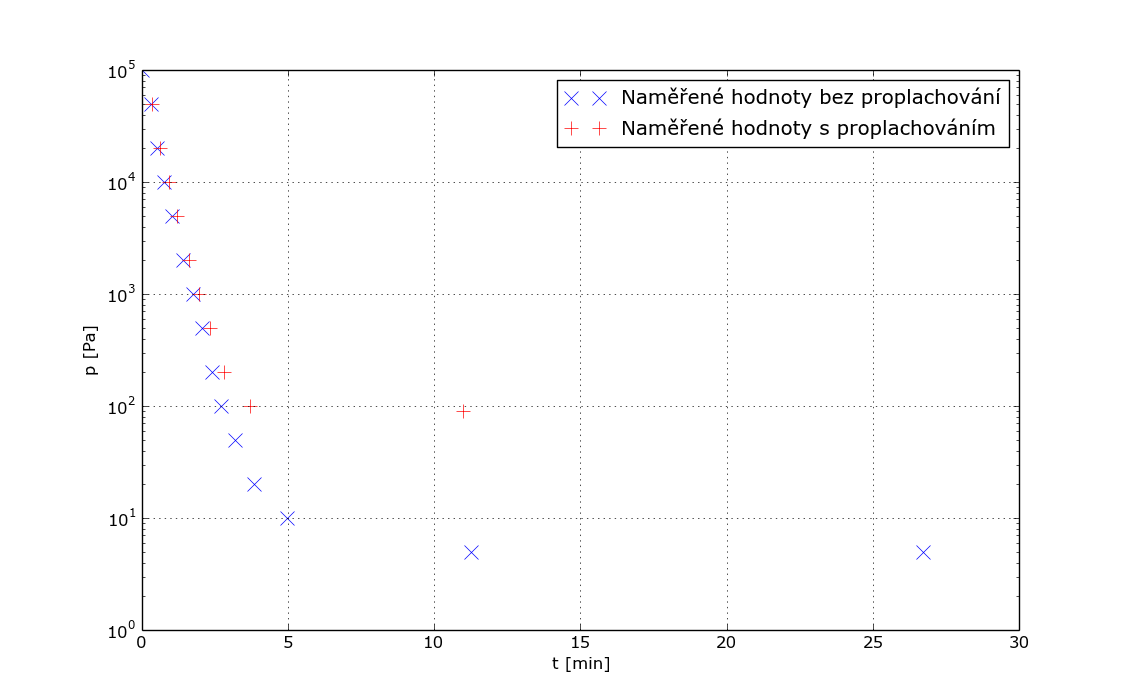
\includegraphics[width=\linewidth]{../pdf/00_p.pdf}
		\vspace*{-0,7cm}
		\caption{Graf závislosti poklesu tlaku na čase při čerpání ROV bez proplachování a s proplachováním.}
		\label{p}
	\end{center}
\end{figure}

\begin{figure}[h!]
	\begin{center}
		\vspace*{-1cm}
		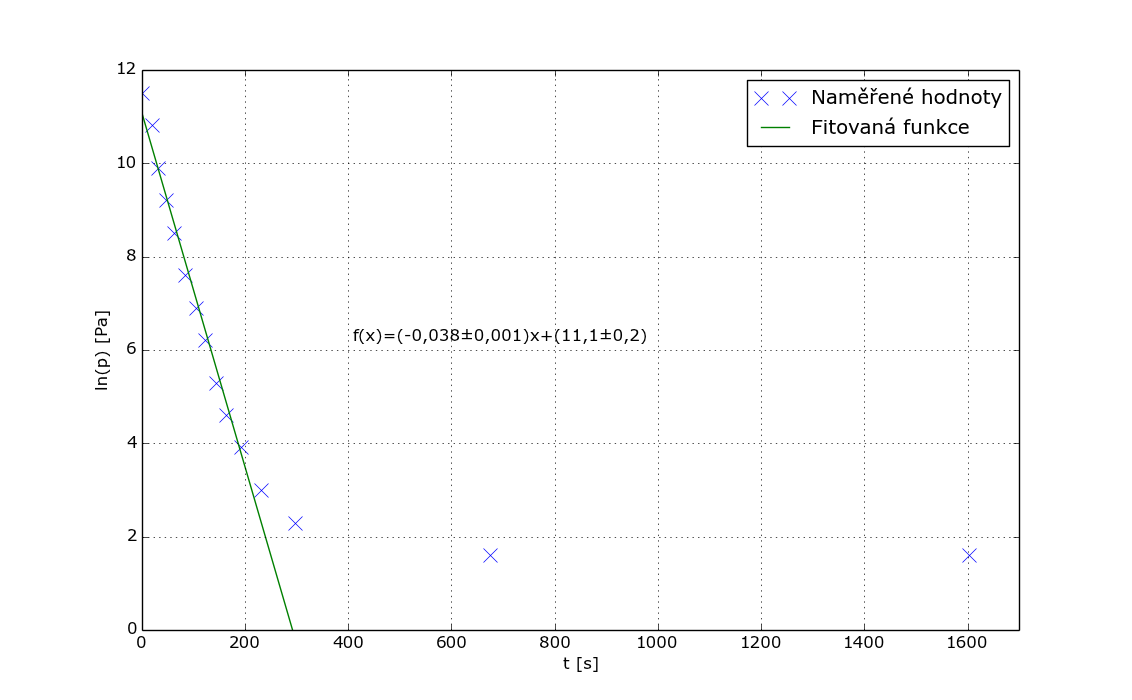
\includegraphics[width=\linewidth]{../pdf/01_lnp.pdf}
		\vspace*{-0,7cm}
		\caption{Graf závislosti ln p na čase při čerpání ROV bez proplachování, graf je proložen lineárním fitem v oblasti $ t = 0-250 $ s.}
		\label{lnp}
	\end{center}
\end{figure}

\begin{figure}[h!]
	\begin{center}
		\vspace*{-1cm}
		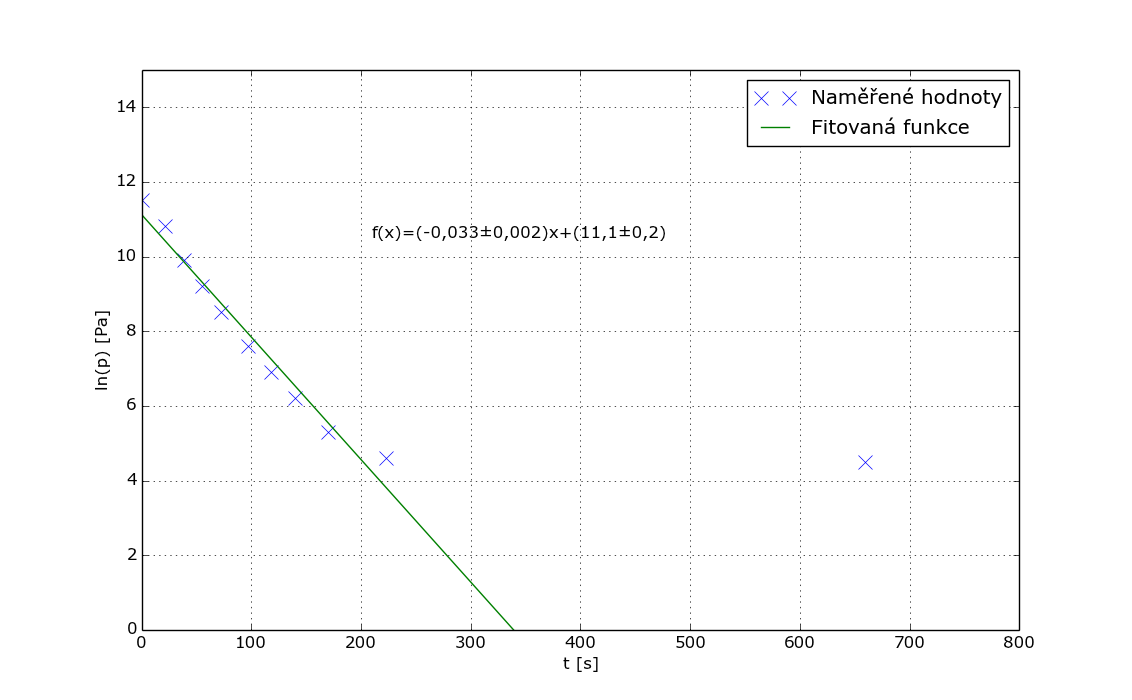
\includegraphics[width=\linewidth]{../pdf/01_lnp_proplach.pdf}
		\vspace*{-0,7cm}
		\caption{Graf závislosti ln p na čase při čerpání ROV s proplachováním, graf je proložen lineárním fitem v oblasti $ t = 0 - 250 $ s.}
		\label{lnp_proplach}
	\end{center}
\end{figure}

\begin{table}[h!]
	\centering
	\begin{tabular}{|r|r|r|r|r|}
		\hline
		$p~\unit{[Pa]}$ & $\tau~\unit{[s]}$ & $l~\unit{[cm]}$ & $\delta V/\delta t~\unit{[mm^3/s]}$ & $S_{EF}~\unit{[cm^3/s]}$ \bigstrut\\
		\hline
		5     & 159,3 & 10    & 3     & 61 \bigstrut\\
		\hline
		10    & 34,5  & 10    & 14    & 140 \bigstrut\\
		\hline
		20    & 14,1  & 10    & 34    & 171 \bigstrut\\
		\hline
	\end{tabular}%
	
	\caption{Naměřené hodnoty pro výpočet efektivní čerpací rychlosti  $S_{EF}$; $ p $ je tlak, $\tau$ je čas, za který olej v mikrobyretě vystoupil o délku $ l $ a $ \delta V $ je objem vzduchu odsátý z mikrobyrety za čas $ \delta t $.}
	\label{efektivni_cerpani}
	
\end{table}


\begin{table}[h!]
	\centering
	\begin{tabular}{|r|r|r|}
		\hline
		$p~\unit{[Pa]}$ & $l_s~\unit{[mm]}$ & $C_{vm}~\unit{[dm^3/s]}$ \bigstrut\\
		\hline
		5     & 1,32  & 2,1 \bigstrut\\
		\hline
		10    & 0,66  & 3,3 \bigstrut\\
		\hline
		15    & 0,44  & 4,6 \bigstrut\\
		\hline
		20    & 0,33  & 5,8 \bigstrut\\
		\hline
		25    & 0,26  & 7,1 \bigstrut\\
		\hline
	\end{tabular}%
	
	\caption{Vypočítané hodnoty pro získání vodivosti trubice $C_{vm} $; $ p $ je tlak, $ l_s $ je střední volná dráha a $C_{vm} $ je vodivost trubice při viskózně molekulárních podmínkách.}
	\label{tab:vodivost}
	
\end{table}

\begin{figure}[h!]
	\begin{center}
		\vspace*{-1cm}
		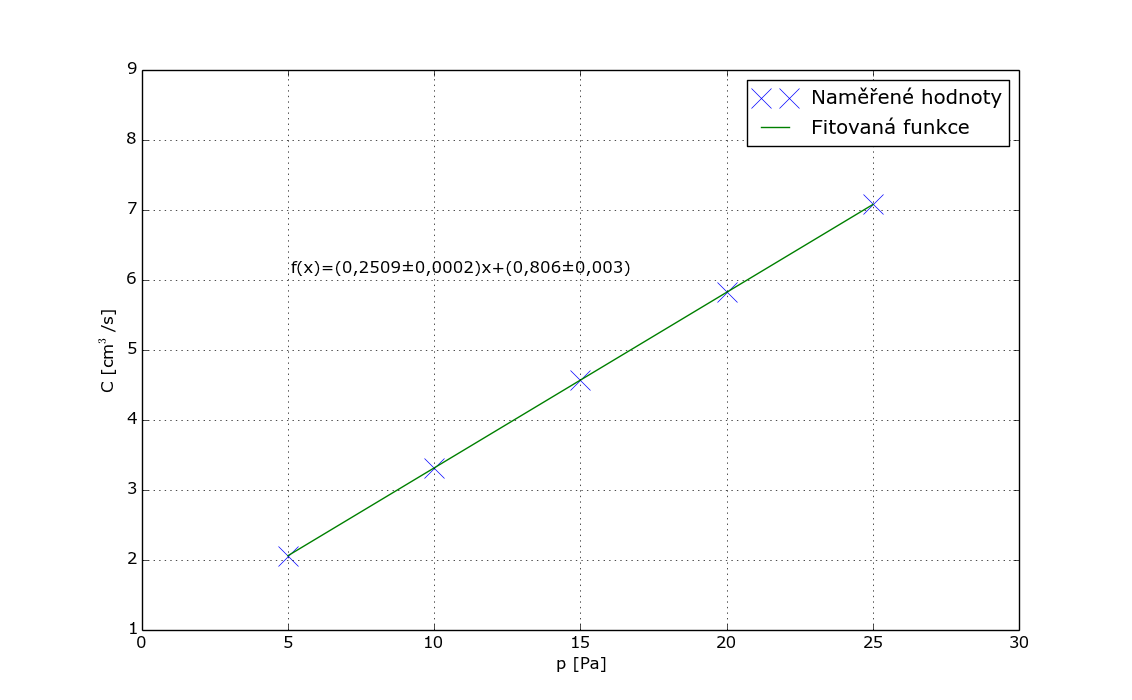
\includegraphics[width=\linewidth]{../pdf/04_vodivost.pdf}
		\vspace*{-0,7cm}
		\caption{Graf závislosti vodivosti trubice mezi ROV a recipientem na tlaku v recipientu.}
		\label{graf_vodivost}
	\end{center}
\end{figure}


\begin{table}[h!]
	\centering
	\begin{tabular}{|r|r|r|r|}
		\hline
		$l~\unit{[mm]}$ & $h~\unit{[mm]}$ & $p~\unit{[Pa]}$ & $n~\unit{[-]}$ \bigstrut\\
		\hline
		7,0   & 5,0   & 4     & 22 \bigstrut\\
		\hline
		8,0   & 6,0   & 6     & 21 \bigstrut\\
		\hline
		9,0   & 7,0   & 8     & 20 \bigstrut\\
		\hline
		10,0  & 8,0   & 10    & 19 \bigstrut\\
		\hline
		11,0  & 9,0   & 12    & 18 \bigstrut\\
		\hline
		11,5  & 9,5   & 13    & 17 \bigstrut\\
		\hline
		12,0  & 10,0  & 15    & 16 \bigstrut\\
		\hline
		12,5  & 10,5  & 16    & 15 \bigstrut\\
		\hline
		14,5  & 12,5  & 22    & 13 \bigstrut\\
		\hline
		16,0  & 14,0  & 28    & 11 \bigstrut\\
		\hline
		20,0  & 18,0  & 44    & 9 \bigstrut\\
		\hline
	\end{tabular}%
	
	
	\caption{Naměřené hodnoty pro cejchování termočlánkového manometru McLeodovým manometrem; $ l $ je vzdálenost mezi vrcholem uzavřené trubice a hladinou v této trubici v McLeodově vakuometru, $ h $ je rozdíl hladin v tomto vakuometru, $ p $ je tlak v recipientu měřený McLeodovým vakuometrem a $n$ je počet dílků na termočlánkovém vakuometru.}
	\label{tab:cejchovani}
	
\end{table}

\begin{figure}[h!]
	\begin{center}
		\vspace*{-2cm}
		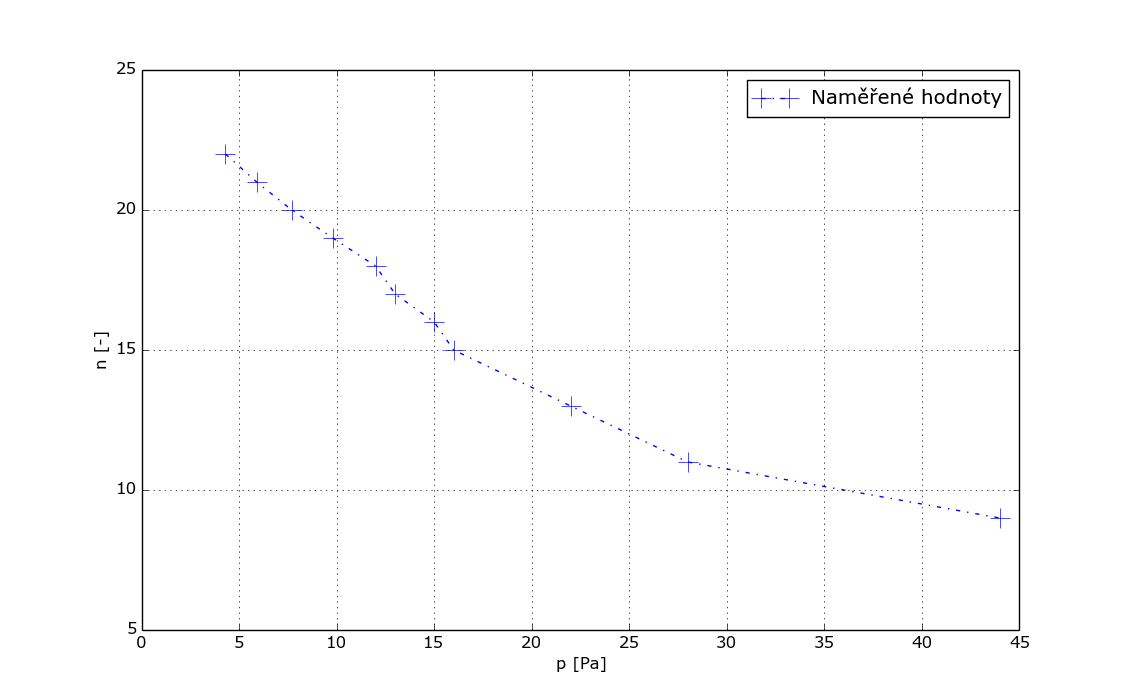
\includegraphics[width=\linewidth]{../pdf/03_cejch.pdf}
		\vspace*{-0,7cm}
		\caption{Cejchování termočlánkového manometru; $ n $ je počet dílků termočlánkového manometru a $ p $ je tlak naměřený McLeodovým vakuometrem.}
		\label{graf_cejchovani}
	\end{center}
\end{figure}


\begin{table}[h!]
	\centering
	\begin{tabular}{|r|r|r|r|r|r|r|r|r|r|}
		\hline
		$l~\unit{[mm]}$ & $h~\unit{[mm]}$ & $p_1~\unit{[Pa]}$ & $n~\unit{[-]}$ & $p_2~\unit{[Pa]}$ & $\tau~\unit{[s]}$ & $\delta V /\delta t~\unit{[mm^3/s]}$ & $p_s~\unit{[Pa]}$ & $C_{vm}~\unit{[cm^3/s]}$ & $C_n~\unit{[cm^3/s]}$ \bigstrut\\
		\hline
		6,5   & 6,5   & 4     & 19    & 10    & 138,4 & 3     & 7     & 98    & 56 \bigstrut\\
		\hline
		7,5   & 7,5   & 5     & 18    & 12    & 112,2 & 4     & 9     & 111   & 61 \bigstrut\\
		\hline
		8,0   & 8,0   & 6     & 16    & 16    & 67,6  & 7     & 11    & 128   & 70 \bigstrut\\
		\hline
		11,0  & 11,0  & 12    & 11    & 28    & 32,5  & 15    & 20    & 190   & 96 \bigstrut\\
		\hline
		13,0  & 13,0  & 18    & 9     & 44    & 17,9  & 27    & 31    & 268   & 100 \bigstrut\\
		\hline
	\end{tabular}%
	
	
	\caption{Naměřené hodnoty pro výpočet vodivosti kovové trubice; $ l $ je vzdálenost mezi vrcholem uzavřené trubice a hladinou v této trubici v McLeodově vakuometru, $ h $ je rozdíl hladin v tomto vakuometru, $ p_1 $ je tlak na začátku trubice měřený McLeodovým vakuometrem, $n$ je počet dílků na termočlánkovém vakuometru,  $ p_2 $ je tlak na konci trubice určený z cejchování termočlánkového manometru, $\tau$ je čas, za který olej v  mikrobyretě vystoupil o $ 10 $ cm, $ \delta V $ je objem vzduchu odsátý z mikrobyrety za čas $ \delta t $, $p_{s}$ je střední tlak v trubici, $C_{n}$ je naměřená vodivost  a  $C_{vm}$ je vypočítaná vodivost.}
	\label{tab:vodivost2}
	
\end{table}

\begin{figure}[h!]
	\begin{center}
		\vspace*{-1cm}
		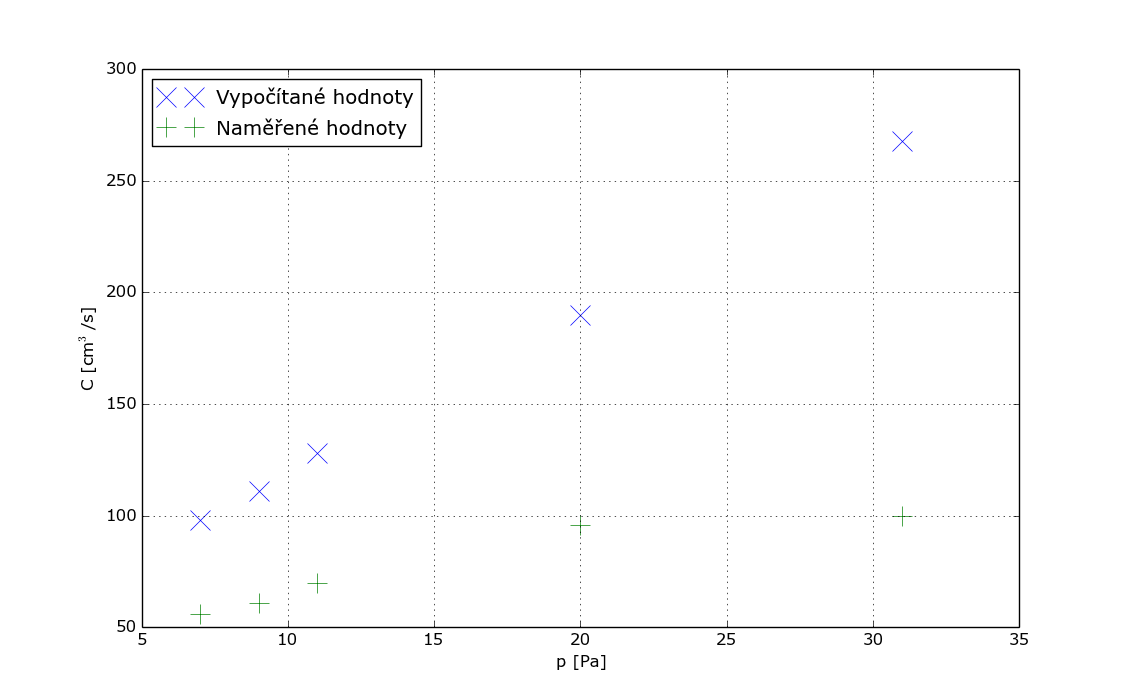
\includegraphics[width=\linewidth]{../pdf/05_cac.pdf}
		\vspace*{-0,7cm}
		\caption{Graf závislost naměřené a vypočítané vodivosti kovové trubice na středním tlaku $ p_s $.}
		\label{graf_vodivost2}
	\end{center}
\end{figure}


%\clearpage
%\subsection{Schémata}
%	
%	\begin{figure}[h!]
%	\centering
%			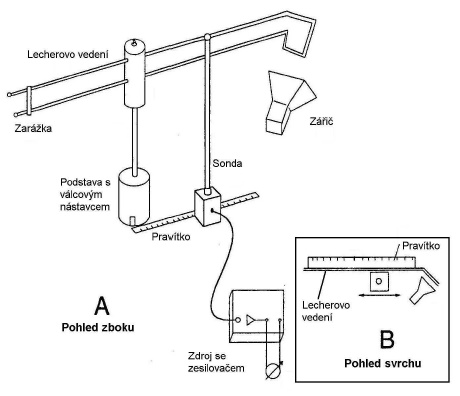
\includegraphics[width=13cm]{att/lecherovo_vedeni.jpg}
%			\caption{Experiment s Lecherovým vedením (převzato z  \cite{bib:zadani}). }
%			\label{fig:lecherovo_vlneni}
%	\end{figure}	
%	
%\clearpage
% --- Konec dokumentu --------------------------------------------------

\end{document}

